\subsection{Features of the tool}
Design documentation expresses the business logic of the WA in a visual fashion by using UML. Main benefit of UML is to allow representation of all the components of a WA by means of diagrams, notations and extension mechanisms. Conallen \cite{cona-02} defined new kinds of elements inside a metamodel and introduced a set of new stereotypes and new icons to represent components like static web pages as well as dynamic ones, frames, forms and to model interactions with databases.

To use UML diagrams in conjunction with Model Checking techniques for performing automatic verification, we implemented a component which is able to automatically translate a WA diagram, exported by an UML tool as XMI file, in the corresponding WAG; then, the WAG is translated in NuSMV code given as input to the model checker. Figure \ref{fig6} shows the location of this component, called \textit{XMI2SMV}, within the tool: 

\begin{figure}[ht]
\centerline{\scalebox{.4}{\includegraphics{figura6.eps}}}
\caption{XMI2SMV component within verification tool \label{fig6}}
\end{figure}

The \textit{XMI2SMV} component includes three packages, according to three principal features it has.

\textbf{XMIManager}. It imports UML diagram as XMI file, then it analyzes XMI file and extracts information about the FSM representing the WA.

More specifically, we reach this goal by means of realization of a \textit{State Table}; it stores relationships between the WA as web system and the same WA as FSM, where states and state transitions respect fundamental principles of the mathematical model.  

The class named ``StateTableCreator''is the main class of the package. It builds the \textit{State Table} by analyzing tags in the \textit{.xmi} document and filling two preliminary tables: \textit{Class Table}, which contains all the classes declared in the XMI file, and \textit{Transition Table}, which contains all declared associations in the XMI file. These two tables include information for building the \textit{State Table}; the ``StateTableCreator'' is able to rebuild the WAG according to XMI model by converting each class and every association in a state or in a state transition of the WAG.

\begin{figure}[ht]
\scalebox{.5}{\includegraphics{classe1.eps}}
\caption{StateTableCreator class \label{fig7}}
\end{figure}

A simple example will make clear the approach:

\footnotesize
\begin{itemize}
	\item every class targeted as ``Server Page'' will become a state labeled as ``action''; 
	\item every class targeted as ``Client Page'' will make both a state labeled as ``page'' and a state labeled as ``window''; 
	\item the declaration of the ``Frameset'' class will elicit elimination of some just created windows, because the corresponding pages are displayed in the same window;  
	\item every association link will become a state labeled as ``link''. 
\end{itemize}

\normalsize
Result is a basic and incomplete WAG: it has only nodes and arcs coming from the State Table. Correctness axioms will be assigned to the nodes by the following Graph Manager package.

\textbf{Graph Manager}. It is the main package of the tool, because it:

\footnotesize
\begin{itemize}
	\item calls main classes of connected packages to start operations like WAG creation or SMV code building;
	\item	manages the labeling of the states in the model according to correctness axioms;
	\item	internally stores WAG by means of suitable data structures, such as an \textit{adjacency matrix} and a \textit{vector of ``nodes''}.
\end{itemize}

\normalsize
More specifically, this package assigns the following labels to each node of the model (according to the fundamental correctness axioms described in previous sections): \textit{firstLoad}, \textit{login} and \textit{logout} which are about mechanisms of user authentication; \textit{error} which is about management of error pages; \textit{none}, \textit{partial} and \textit{all} which are about accessibility of private pages. 

However, to identify the states satisfying the above properties, the \textit{Graph Manager} needs information about main pages of WA. Hence WA designers have to provide a XML file, containing names of: homepage,	registration server page, both login and logout server pages, private pages displayed after either administrator or user login (and linked to logout page), error pages and so on. Each name is used by a function of ``Setting'' class; it selects the node of the graph corresponding to a specific web page and assigns to it the label related to the appropriate axiom of correctness.  

To inspect the graph or to select a specific node, the \textit{Graph Manager} exploits its internal model of the WAG. It is based on two special structures: an \textit{adjacency matrix}, where are stored --for each node-- information about connections with adjacent nodes, and a \textit{vector of ``Nodes''}, where each ``Node'' is a vector containing the name of the specific node followed by labels of the axioms of correctness.

Finally, when WAG is completed, ``addSpecification'' function allows to add \ctl specifications to the model; hence for each specification, ``WagManager'' class initializes a new class ``Specification'' and stores \ctl specifications in its \textit{formula} field.

%\begin{figure}[ht]
%\centerline{\scalebox{.5}{\includegraphics{classe2.eps}}}
%\caption{Graph and Node structures used in Graph Manager package \label{fig8}}
%\end{figure}

\textbf{SMVManager}. The third package of the tool builds the SMV code related to the WA, whose model and \ctl specifications are provided by the \textit{Graph Manager}. ``SMVGenerator'' is the main class of the package and coordinates following actions:

\footnotesize
\begin{itemize}
	\item	analysis of all the WAG states to obtain information useful for the translation of the model in the corresponding NuSMV formalism;
	\item	building and syntactic arrangement of \textit{MAIN} module contents modeling the WA states;
	\item	building and syntactic arrangement of the further \textit{SYNCHRO} module contents modeling the user state;
	\item	adding of the correctness axioms in the \textit{MAIN} module;
	\item	performing the SMV code automatic verification.
\end{itemize}

%\begin{figure}[ht]
%\centerline{\scalebox{.5}{\includegraphics{classe3.eps}}}
%\caption{SMVGenerator class \label{fig9}}
%\end{figure}

\normalsize
As previously stated, to perform such actions, the package is equipped with a XML file, containing information to be inserted in SMV code and related to every WAG. 